% THIS DOCUMENT IS TAILORED TO REQUIREMENTS FOR SCIENTIFIC COMPUTING.  IT SHOULDN'T
% BE USED FOR NON-SCIENTIFIC COMPUTING PROJECTS
\documentclass[12pt]{article}

\usepackage{amsmath, mathtools}
\usepackage{amsfonts}
\usepackage{amssymb}
\usepackage{graphicx}
\usepackage{colortbl}
\usepackage{xr}
\usepackage{hyperref}
\usepackage{longtable}
\usepackage{xfrac}
\usepackage{tabularx}
\usepackage{float}
\usepackage{siunitx}
\usepackage{booktabs}
\usepackage{caption}
\usepackage{pdflscape}
\usepackage{afterpage}
\usepackage{enumitem}

\usepackage[round]{natbib}

%\usepackage{refcheck}

\hypersetup{
    bookmarks=true,         % show bookmarks bar?
      colorlinks=true,       % false: boxed links; true: colored links
    linkcolor=red,          % color of internal links (change box color with linkbordercolor)
    citecolor=green,        % color of links to bibliography
    filecolor=magenta,      % color of file links
    urlcolor=cyan           % color of external links
}

%% Comments

\usepackage{color}

\newif\ifcomments\commentstrue %displays comments
%\newif\ifcomments\commentsfalse %so that comments do not display

\ifcomments
\newcommand{\authornote}[3]{\textcolor{#1}{[#3 ---#2]}}
\newcommand{\todo}[1]{\textcolor{red}{[TODO: #1]}}
\else
\newcommand{\authornote}[3]{}
\newcommand{\todo}[1]{}
\fi

\newcommand{\wss}[1]{\authornote{magenta}{SS}{#1}} 
\newcommand{\plt}[1]{\authornote{cyan}{TPLT}{#1}} %For explanation of the template
\newcommand{\an}[1]{\authornote{cyan}{Author}{#1}}

%% Common Parts

\newcommand{\progname}{Software Engineering} % PUT YOUR PROGRAM NAME HERE
\newcommand{\authname}{Team \#5, Money Making Mauraders
\\ Zhenia Sigayev
\\ Justin Ho
\\ Thomas Wang
\\ Michael Shi
\\ Johnny Qu
}


\usepackage{hyperref}
    \hypersetup{colorlinks=true, linkcolor=blue, citecolor=blue, filecolor=blue,
                urlcolor=blue, unicode=false}
    \urlstyle{same}
                                


% For easy change of table widths
\newcommand{\colZwidth}{1.0\textwidth}
\newcommand{\colAwidth}{0.13\textwidth}
\newcommand{\colBwidth}{0.82\textwidth}
\newcommand{\colCwidth}{0.1\textwidth}
\newcommand{\colDwidth}{0.05\textwidth}
\newcommand{\colEwidth}{0.8\textwidth}
\newcommand{\colFwidth}{0.17\textwidth}
\newcommand{\colGwidth}{0.5\textwidth}
\newcommand{\colHwidth}{0.28\textwidth}

% Used so that cross-references have a meaningful prefix
\newcounter{defnum} %Definition Number
\newcommand{\dthedefnum}{GD\thedefnum}
\newcommand{\dref}[1]{GD\ref{#1}}
\newcounter{datadefnum} %Datadefinition Number
\newcommand{\ddthedatadefnum}{DD\thedatadefnum}
\newcommand{\ddref}[1]{DD\ref{#1}}
\newcounter{theorynum} %Theory Number
\newcommand{\tthetheorynum}{TM\thetheorynum}
\newcommand{\tref}[1]{TM\ref{#1}}
\newcounter{tablenum} %Table Number
\newcommand{\tbthetablenum}{TB\thetablenum}
\newcommand{\tbref}[1]{TB\ref{#1}}
\newcounter{assumpnum} %Assumption Number
\newcommand{\atheassumpnum}{A\theassumpnum}
\newcommand{\aref}[1]{A\ref{#1}}
\newcounter{goalnum} %Goal Number
\newcommand{\gthegoalnum}{GS\thegoalnum}
\newcommand{\gsref}[1]{GS\ref{#1}}
\newcounter{instnum} %Instance Number
\newcommand{\itheinstnum}{IM\theinstnum}
\newcommand{\iref}[1]{IM\ref{#1}}
\newcounter{reqnum} %Requirement Number
\newcommand{\rthereqnum}{R\thereqnum}
\newcommand{\rref}[1]{R\ref{#1}}
\newcounter{nfrnum} %NFR Number
\newcommand{\rthenfrnum}{NFR\thenfrnum}
\newcommand{\nfrref}[1]{NFR\ref{#1}}
\newcounter{lcnum} %Likely change number
\newcommand{\lthelcnum}{LC\thelcnum}
\newcommand{\lcref}[1]{LC\ref{#1}}

\usepackage{fullpage}

\begin{document}

\title{Software Requirements Specification for \progname: MES Finance Tracking Platform} 
\author{\authname}
\date{\today}
	
\maketitle

~\newpage

\pagenumbering{roman}

\tableofcontents

~\newpage

\section*{Revision History}

\begin{tabularx}{\textwidth}{p{3cm}p{2cm}X}
  \toprule {\bf Date} & {\bf Version} & {\bf Notes}\\
    \midrule
      Date 1 & 1.0 & Notes\\
      Date 2 & 1.1 & Notes\\
  \bottomrule
\end{tabularx}

\newpage
\pagenumbering{arabic}


%-------------------------------------
% 1. Purpose of the Project
%-------------------------------------
\section{Purpose of the Project - Thomas}
  \subsection{User Business - Thomas}
    The McMaster Engineering Society (MES) seeks a more effective and efficient way to manage and track finances of its over 60 student clubs. Due to the current difficuties of 
    the manual proces to manage and track reimbursements, the MES needs to streamline the process so reimbursements can occur regularly throughout the year and have them processed
    quicker to reduce processing times for students. The implementation of our solution will allow student clubs to submit reimbursement requests digitally and in an easier manner, 
    allow MES reviewers to approve or reject requests efficiently, and provide transparency to all parties involved in the reimbursement process. 

  \subsection{Goals of the Project - Thomas}
    The primary goals of the MES Finance Tracking Platform are to:
    \begin{itemize}
      \item Provide a user-friendly interface for club members to submit expense reimbursement requests.
      \item Implement a robust review and approval workflow for MES staff to manage reimbursement requests efficiently.
      \item Ensure transparency and traceability of all financial transactions related to club reimbursements.
      \item Maintain data security and privacy in compliance with McMaster University policies.
      \item Integrate seamlessly with existing MES systems and infrastructure.
    \end{itemize}

%-------------------------------------
% 2. System Overview
%-------------------------------------
\section{System Overview}

  \subsection{Architecture Diagram}
    \begin{figure}[H]
        \centering
        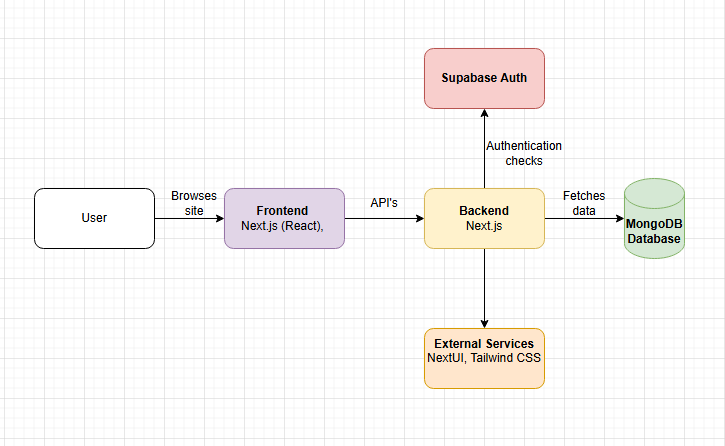
\includegraphics[width=0.8\textwidth]{architecture_diagram_Justin.png}
        % \caption{TODO: ADD CAPTION FOR ARCHITECTURE DIAGRAM. This should be a general overview of the flow of information and how 
        % features interact with each other. No technologies etc should be included here.}
        \label{fig:architecture_diagram}
    \end{figure}

  \subsection{Technology Stack Overview}
    The system is a web-based application built with modern JavaScript frameworks and libraries, designed to support the needs of the MacEng Society website. The application provides user-facing web pages and administrative features for content management. It is structured as a client-server application where the frontend runs in a web browser and the backend interacts with a database.
    \subsection{Frontend (Client-Side)}
    \begin{itemize}
        \item Developed using \textbf{React/Next.js}.
        \item Runs in modern web browsers such as Google Chrome, Microsoft Edge, Firefox, and Safari.
        \item Provides the user interface for interacting with content such as council information, events, and bookings.
        \item Fetches and displays data from the backend via RESTful or GraphQL APIs.
    \end{itemize}

    \subsection{Backend (Server-Side)}
    \begin{itemize}
        \item Executes on the \textbf{Node.js} runtime environment.
        \item Manages application logic, routing, and communication with the database.
        \item Uses \textbf{MongoDB Community Server} as the primary data storage system.
        \item Exposes APIs consumed by the frontend for dynamic content delivery.
    \end{itemize}

    \subsection{Database}
    \begin{itemize}
        \item Implemented using \textbf{MongoDB Community Server}.
        \item Stores member information, content, and other structured data required for the application.
    \end{itemize}

    \subsection{Development Environment}
    \begin{itemize}
        \item Source code is managed using \textbf{Git} and hosted in a repository such as GitHub.
        \item Developers use \textbf{Visual Studio Code (VSCode)} with mandatory extensions:
        \begin{itemize}
            \item ESLint
            \item Prettier
        \end{itemize}
        \item Project dependencies are managed with \textbf{pnpm} or \textbf{yarn}.
        \item \textbf{Husky} and linting hooks enforce branch naming conventions, commit message standards, and code consistency.
    \end{itemize}

    \subsection{External Dependencies}
    \begin{itemize}
        \item \textbf{GitHub Actions} (via \texttt{.github/workflows}) for CI/CD and automated testing.
        \item \textbf{NextUI} and \textbf{TailwindCSS} for UI components and styling.
        \item Additional \textbf{Node.js} ecosystem libraries and packages installed via pnpm or yarn.
    \end{itemize}

    % \begin{figure}[H]
    %     \centering
    %     
\includegraphics[width=0.8\textwidth]{tech_stack.png}
    %     \caption{TODO: ADD CAPTION FOR TECH STACK OVERVIEW. This should be a general overview of the technologies used in the system and how they interact with each other.
    %     This should show how the frontend and backend interact with each other and any external services used.}
    %     \label{fig:tech_stack_overview}
    % \end{figure}

%-------------------------------------
% 3. Stakeholders
%-------------------------------------
\section{Stakeholders - Thomas}
  \subsection{Direct Stakeholders}
    \subsubsection{Club Leadership}
      \begin{itemize}
        \item \textbf{Description}: Members of the executive team of clubs that fall under the MES.  
        \item \textbf{Use Cases:}
          \begin{itemize}
            \item Review and submit expense reimbursement requests on behalf of their club.
            \item Track the status of submitted requests.
            \item Review past reimbursements and budget accordingly
          \end{itemize}
      \end{itemize}
    \subsubsection{Club General Members}
      \begin{itemize}
        \item \textbf{Description}: General members of clubs that fall under the MES.
        \item \textbf{Use Cases:}
          \begin{itemize}
            \item Submit expense reimbursement requests for expenses incurred on behalf of their club, pending review of executives.
          \end{itemize}
      \end{itemize}
    \subsubsection{McMaster University Finance}
      \begin{itemize}
        \item \textbf{Description}: University staff responsible for auditing and overseeing the financial activities of student organizations.
        \item \textbf{Use Cases:}
          \begin{itemize}
            \item Issue reimbursements to club members based on approved requests.
            \item Ensure compliance with university financial policies and regulations.
          \end{itemize}
      \end{itemize}

  \subsection{Indirect Stakeholders}
    \subsubsection{MES}
      \begin{itemize}
        \item \textbf{Description}: Owns the platform and is responsible for the longterm sustainability, governance, and decisions regarding the platform.
        \item \textbf{Use Cases:}
          \begin{itemize}
            \item Benefit from well-managed clubs and events funded through the MES.
            \item Access information about club activities and financial transparency.
          \end{itemize}
      \end{itemize}
    \subsubsection{MES Student Developers}
      \begin{itemize}
        \item \textbf{Description}: Students hired by the MES to maintain and improve the MES platform, including the finance tracking system.
        \item \textbf{Use Cases:}
          \begin{itemize}
            \item Maintain and update the finance tracking platform as needed.
            \item Ensure the platform remains secure, reliable, and user-friendly.
          \end{itemize}
      \end{itemize}

  \subsection{Personas - Thomas}
    \begin{itemize}
      \item Wayne, Club President (Age 21): Looking for time-saving way to submit reimbursements
      \item Alice, Club Member (Age 20): Wants to easily submit expenses for club activities
      \item Frank, Club VP Finance (Age 21): Needs transparency into club spending and budgets
      \item Bob, MES Reviewer (Age 25): Needs efficient way to review and approve requests
      \item Eve, MES Admin (Age 30): Wants to ensure system is secure and compliant
      \item Charlie, MES Developer (Age 22): Needs maintainable and well-documented codebase
    \end{itemize}
  \subsection{Priorities Assigned to Stakeholders - Thomas}
    \begin{itemize}
      \item Key Users: Club Leadership; would like a easy way to submit and track reimbursements
      \item Secondary Users: MES Administrators; would like to ensure a secure and compliant way to manage and deliver reimbursements
      \item Tertiary Users: Casual Users; requirements are low priority
    \end{itemize}
  \subsection{Stakeholder Participation - Thomas}
    \begin{itemize}
      \item Gathering Requirements: Conduct interviews and surveys with club leaders and MES staff to understand key needs and an understanding of the current process and the desired changes.
      \item Usability Testing: Tangible session to validate and observe the usability of the platform with real users. 
      \item Feedback and Iteration: Regularly gather feedback from stakeholders during development to ensure the platform meets their needs.
      \item Training and Support: Provide training sessions and support materials to help stakeholders effectively use the platform.
      \item Ongoing Engagement: Maintain open communication channels for continuous feedback and improvement after deployment.
    \end{itemize}


%-------------------------------------
% 4. Mandated Constraints
%-------------------------------------
\section{Mandated Constraints}


\subsection{Solution Constraints}
  \begin{enumerate}
    \item The system must be capable of managing expense reimbursement requests for up to 61 clubs or 7000 students.
    \item The system must track and display the real-time status of each reimbursement request (e.g., submitted, under review, approved, rejected, reimbursed) to ensure transparency for submitters, reviewers, and administrators.
    \item The system must allow users to attach digital receipts in PDF or image formats to their reimbursement requests.
    \item The system must comply with data privacy regulations, ensuring that all personal and financial information is securely stored and transmitted.
    \item The system must be able to import existing financial data from the current MES finance tracker to ensure continuity and data integrity.
    \item The system must maintain consistent in accordance with the overall MES platform availability to support uninterrupted access.
  \end{enumerate}

\subsection{Current MES Finance Tracker}
  \begin{itemize}
    \item \textbf{MC X:}
      \begin{itemize}[label=$\circ$]
        \item \textbf{description:} The current MES finance tracker is not scalable and lacks proper traceability features.
        \item \textbf{rationale:} The new system must be designed to integrate with existing MES infrastructure and address current limitations.
      \end{itemize}
  \end{itemize}

\subsection{Cost Constraints}
  \begin{itemize}
    \item \textbf{MC X:}
      \begin{itemize}[label=$\circ$]
        \item \textbf{description:} The amount spent by a team should not exceed \$500.
        \item \textbf{rationale:} The project must meet capstone budget constraints and be economically feasible for MES to support and maintain.
      \end{itemize}
  \end{itemize}

\subsection{Off-the-Shelf Software}
  \begin{itemize}
    \item \textbf{MC X:}
      \begin{itemize}[label=$\circ$]
        \item \textbf{description:} There are other financial tracking options (e.g., Quickbooks), but they may not match MES look-and-feel or budget.
        \item \textbf{rationale:} Ensures the chosen solution integrates seamlessly with MES UX and licensing constraints.
      \end{itemize}
  \end{itemize}

\subsection{Schedule Constraints}
  \begin{itemize}
    \item \textbf{MC X:}
      \begin{itemize}[label=$\circ$]
        \item \textbf{description:} The project must be completed by March 2026.
        \item \textbf{rationale:} Allows deployment one month before term end to avoid an end-of-term submission surge.
      \end{itemize}
  \end{itemize}

\subsection{Workflow Constraints}
  \begin{itemize}
    \item \textbf{MC X:}
      \begin{itemize}[label=$\circ$]
        \item \textbf{description:} Capstone group will collaborate with MES developers using staging branches and incremental merges.
        \item \textbf{rationale:} Minimizes disruption and enables gradual adoption.
      \end{itemize}
  \end{itemize}

\subsection{Enterprise Constraints}
  \begin{itemize}
    \item \textbf{MC X:}
      \begin{itemize}[label=$\circ$]
        \item \textbf{description:} Development must use technologies with favourable licensing terms for non-profits.
        \item \textbf{rationale:} Avoids licensing costs or obligations that could hinder MES future plans.
      \end{itemize}
  \end{itemize}


%-------------------------------------
% 5. Terminology, Acronyms, and Technologies
%-------------------------------------
\section{Terminology, Acronyms, and Technologies}

  \subsection{Terminology}
    \begin{itemize}
      \item \textbf{Audit Log}: A chronological record of all changes made to the system, including who made the change and when it was made.
      \item \textbf{Budget Allocation}: The total amount of funds allocated to a club or team for a specific period, typically a fiscal year.
      \item \textbf{Expense Claim}: A request for reimbursement submitted by a club or team member for expenses incurred on behalf of the club or team.
      \item \textbf{Receipt}: A digital or physical document that serves as proof of purchase for an expense.
      \item \textbf{Reimbursement}: The process of repaying a club or team member for approved expenses.
      \item \textbf{Reviewer}: An MES staff member or administrator responsible for reviewing and approving or rejecting expense claims.
      \item \textbf{Submitter}: A club or team member who submits an expense claim for reimbursement.
      \item \textbf{MES Administrator}: An MES staff member with elevated permissions to manage the finance tracking platform, including user roles and system settings.
    \end{itemize}

  \subsection{Acronyms}
    \begin{itemize}
      \item \textbf{MES:} McMaster Engineering Society.
        \begin{itemize}[label=$\circ$]
          \item \textbf{description:} The student-led organization representing engineering students at McMaster University.
        \end{itemize}
      \item \textbf{SLA:} Service Level Agreement.
        \begin{itemize}[label=$\circ$]
          \item \textbf{description:} A formal agreement between a service provider and a client that outlines the expected level of service.
        \end{itemize}
      \item \textbf{CI:} Content Integration.
        \begin{itemize}[label=$\circ$]
          \item \textbf{description:} Content integration refers to validating the correctness of the software changes, typically running unit or integration tests.
        \end{itemize}
      \item \textbf{CD:} Content Deployment.
        \begin{itemize}[label=$\circ$]
          \item \textbf{description:} Content deployment refers to deploying those changes to your product / platform (e.g., a website) for users to interact with.
        \end{itemize}
      \item \textbf{CTA:} Call-to-Action.
        \begin{itemize}[label=$\circ$]
          \item \textbf{description:} An element of a web-page (e.g., a button or link) that encourages users to take a specific action.
        \end{itemize}
      \item \textbf{UX:} User Experience.
        \begin{itemize}[label=$\circ$]
          \item \textbf{description:} The overall experience a user has when interacting with a product, including usability and design.
        \end{itemize}
      \item \textbf{UI:} User Interface.
        \begin{itemize}[label=$\circ$]
          \item \textbf{description:} The visual and interactive elements users interact with (buttons, menus, forms).
        \end{itemize}
      \item \textbf{OCR:} Optical Character Recognition.
        \begin{itemize}[label=$\circ$]
          \item \textbf{description:} Technology that converts images of text into editable and searchable data.
        \end{itemize}
      \item \textbf{WCAG:} Web Content Accessibility Guidelines.
        \begin{itemize}[label=$\circ$]
          \item \textbf{description:} Guidelines from W3C to make web content more accessible to people with disabilities.
        \end{itemize}
    \end{itemize}

  \subsection{Technologies}
    \begin{itemize}
      \item \textbf{Front-end:} The client-side part of the application that users interact with directly, typically built using HTML, CSS, and JavaScript frameworks.
      \item \textbf{Back-end:} The server-side part of the application that handles business logic, database interactions, and authentication, often built using languages like Python, Ruby, or Node.js.
      \item \textbf{Full-Stack:} A combination of both front-end and back-end development, where a developer is proficient in working on all layers of the application.
      \item \textbf{Testing:} The process of evaluating the functionality and performance of the application to ensure it meets the specified requirements and is free of defects.
      \item \textbf{Database:} A structured collection of data that is stored and managed to facilitate efficient retrieval and manipulation.
      \item \textbf{Cloud Services:} Online platforms that provide computing resources, storage, and services over the internet, such as AWS, Azure, or Google Cloud.
      \item \textbf{Version Control:} A system that tracks changes to code and allows multiple developers to collaborate on a project, with Git being the most popular version control system.
    \end{itemize}

%-------------------------------------
% 6. Relevant Facts And Assumptions
%-------------------------------------
\section{Relevant Facts And Assumptions - Michael}
  \subsection{Relevant Facts - Michael}
  \subsection{Business Rules - Michael}
  \subsection{Assumptions - Michael}

%-------------------------------------
% 7. The Scope of the Work
%-------------------------------------
\section{The Scope of the Work - Michael}
  \subsection{The Current Situation - Michael}
    The MES currently uses spreadsheets and manual processes
    to track club finances. This approach often results in errors from lost receipts,
    duplicated claims, and large amounts of claims at the end of the year. A centralized
    financial tracking platform is needed to streamline and automate
    this process for the MES.

  \subsection{The Context of the Work - Michael}
  \subsection{Work Partitioning - Michael}
  \subsection{Specifying a Business Use Case (BUC) - Michael}

%-------------------------------------
% 8. Business Data Model and Data Dictionary
%-------------------------------------
\section{Business Data Model and Data Dictionary - Thomas}
  \subsection{Business Data Model - Thomas}
  \begin{itemize}
    \item MES Admin User Entity:
      \begin{itemize}
        \item \textbf{Description:} An individual associated with McMaster that verifies, validates, and administers the reimbursements
        \item \textbf{Attributes:} Name, Email, roleID, Phone Number
        \item \textbf{Relationship:} MES Admin may approve, reject, request additional information, and administer reimbursements 
      \end{itemize}
    
    \item Club Admin + General User Entity:
      \begin{itemize}
          \item \textbf{Description:} Members apart of a MES club who wishes to submit items for reimbursements
          \item \textbf{Attributes:} Name, macID, Email, clubID, roleID, Phone Number
          \item \textbf{Relationship:} A club member may submit multiple reimbursement requests. Specified club admin team role grants permission to finalize reimbursement request on behalf of the club
        \end{itemize}

    \item Club Entity:
      \begin{itemize}
          \item \textbf{Description:} Club Entity that consists of all club members/those who will be creating reimbursement requests
          \item \textbf{Attributes:} clubID, clubName
          \item \textbf{Relationship:} A club entity that submits request on behalf of the club. Members within club entity can be added or removed (only for people with club admin team role)
        \end{itemize}
    
    \item Reimbursement Request Entity:
      \begin{itemize}
          \item \textbf{Description:} Reimbursement request that has been approved by club leadership and submitted to MES admin team for review
          \item \textbf{Attributes:} clubID, requestID, Timestamp, amountRequested, requesetStatus, attachments(recipets)
          \item \textbf{Relationship:} A request is linked to a particular club, MES admin team can review the reimbursement and change its status between approved, rejected, pending
        \end{itemize}
    
    \item Budget Entity:
      \begin{itemize}
          \item \textbf{Description:} Data displayed for budget allocated by MES to a particular club 
          \item \textbf{Attributes:} clubID, totalAmountAllocated, totalAmountSpent, pendingAmount
          \item \textbf{Relationship:} A display of the total resources available for a club 
        \end{itemize}

    \item Role Entity:
      \begin{itemize}
          \item \textbf{Description:} List of all roles that can be assigned to an individual
          \item \textbf{Attributes:} roleID, roleName
          \item \textbf{Relationship:} Every person at McMaster has an account, no default role assigned. Roles will be later assigned
        \end{itemize}
  \end{itemize}
  \subsection{Data Dictionary - Thomas}
  N/A (No data dictionary information at this time).

%-------------------------------------
% 9. Functional Requirements
%-------------------------------------
\section{Functional Requirements}
  \subsection{Functional Requirements}
    \begin{itemize}
      \item The system shall allow MES clubs and teams to submit expense claims.
      \item The system shall provide MES reviewers with tools to efficiently review, approve, or reject the reimbursement requests.
      \item The system shall track the status of each expense claim (e.g., submitted, under review, approved, rejected, reimbursed).
      \item The system shall permanently store and retain digital receipt submissions.
      \item The system shall maintain an audit trail that records who submitted, reviewed, approved, or denied each expense claim.
      \item The system shall enable access to club expense submissions to the submitters, and other club members with a role greater or equal to that of the submitter, or MES administrators and approvers.
    \end{itemize}

%-------------------------------------
% 10. Non-Functional Requirements
%-------------------------------------
\section{Non-Functional Requirements}

The following 7 sections outline the non-functional requirements for the MES Finance Tracking Platform.

%-------------------------------------
% 11. Look and Feel Requirements
%-------------------------------------
\section{Look and Feel Requirements}
    \subsection{Appearance Requirements}
    \begin{itemize}
        \item The interface should use the McMaster Engineering Society’s branding colors and logo.
        \item The design should maintain a clean, modern layout using NextUI and TailwindCSS for consistency.
        \item The application should use responsive design principles to adapt to desktop, tablet, and mobile displays.
        \item Buttons, icons, and navigation components should follow accessible contrast ratios (WCAG 2.1 AA).
    \end{itemize}

    \subsection{Style Requirements}
    \begin{itemize}
        \item Typography should match MES branding guidelines, using sans-serif fonts for readability.
        \item UI components must adhere to consistent padding, spacing, and rounded-corner styles.
        \item Notification banners and status indicators (e.g., “Submitted,” “Pending,” “Approved”) should use color cues for clarity.
        \item The application should provide a visually appealing balance between white space and content density.
    \end{itemize}
%-------------------------------------
% 12. Usability and Humanity Requirements
%-------------------------------------
\section{Usability and Humanity Requirements}
  \subsection{Ease of Use and Learning Requirements}
    \begin{itemize}
      \item A straightforward optional overview or tutorial should be provided to first-time users.
    \end{itemize}

  \subsection{Personalization and Internationalization Requirements}
    \begin{itemize}
      \item The platform will be in English only.
    \end{itemize}

  \subsection{Understandability and Politeness Requirements}
    \begin{itemize}
      \item The platform will not use offensive language, imagery, symbols, or media of any kind.
      \item All errors and warnings will be communicated in a clear, concise, and polite manner.
    \end{itemize}

  \subsection{Accessibility Requirements}
    \begin{itemize}
      \item Front-end navigation and interactions must comply with WCAG standards to ensure accessibility for users with disabilities.
      \item The platform will allow users to select between light and dark mode themes.
      \item The front-end will use semantic tags (<header>, <main>, <nav>, <footer>, <article>, <button>, etc.) for structure.
      \item All images must have meaningful alternative text (alt).
      \item All functionality must be navigable from a keyboard (i.e., tab to move through content).
    \end{itemize}

%-------------------------------------
% 13. Performance Requirements
%-------------------------------------
\section{Performance Requirements}
  \subsection{Speed and Latency Requirements}
    \begin{itemize}
        \item API response times must average below 1 second for standard database queries and data submissions.
        \item Page load times should not exceed 3 seconds under normal operating conditions on modern browsers.
        \item File uploads (e.g., receipts or invoices) must complete within 5 seconds for files under 10 MB.
    \end{itemize}

  \subsection{Safety-Critical Requirements}
    \begin{itemize}
        \item The system must ensure that no reimbursement or financial transaction is executed without MES reviewer approval.
        \item All monetary data must be validated before submission to prevent corruption or duplication.
    \end{itemize}

  \subsection{Precision or Accuracy Requirements}
    \begin{itemize}
        \item Financial transactions must maintain accuracy up to two decimal places.
        \item All calculations involving funding allocations or reimbursements must be precise and consistent with MES accounting standards.
    \end{itemize}

  \subsection{Robustness or Fault-Tolerance Requirements}
    \begin{itemize}
        \item The system should handle unexpected backend or network failures gracefully, displaying meaningful error messages to users.
        \item Data must be saved incrementally to prevent loss during unexpected session timeouts or browser crashes.
        \item In the event of a failed API request, the system should automatically retry up to three times before reporting failure.
    \end{itemize}

  \subsection{Capacity Requirements}
    \begin{itemize}
        \item The system must support at least 500 concurrent users without noticeable degradation in performance.
        \item The database must handle storage for at least 10,000 user records and 100,000 expense claims.
    \end{itemize}

  \subsection{Scalability or Extensibility Requirements}
    \begin{itemize}
        \item The system must be designed to allow horizontal scaling (e.g., deploying additional backend instances during high usage).
        \item New features such as additional modules (e.g., club budgeting or analytics dashboards) should be easily integrable without major architectural changes.
    \end{itemize}

  \subsection{Longevity Requirements}
    \begin{itemize}
        \item The system is expected to remain operational and maintainable for at least 5 years with regular updates.
        \item Future technology stack upgrades (React, Node.js, MongoDB versions) should not require a full system rewrite.
    \end{itemize}

%-------------------------------------
% 14. Operational and Environmental Requirements
%-------------------------------------
\section{Operational and Environmental Requirements}
  \subsection{Expected Physical Environment}
    \begin{itemize}
      \item The system will be accessed through desktop and laptop computers using modern browsers (Chrome, Edge, Firefox, Safari).
      \item Users may also access the site via tablets or smartphones with stable internet connectivity.
    \end{itemize}

  \subsection{Wider Environment Requirements}
    \begin{itemize}
      \item The application will be hosted on cloud infrastructure (e.g., Vercel or AWS) with automatic scaling and uptime monitoring.
      \item The system must operate effectively under typical university network conditions, including campus Wi-Fi and VPN connections.
    \end{itemize}

  \subsection{Requirements for Interfacing with Adjacent Systems}
    \begin{itemize}
      \item The system may integrate with McMaster’s Single Sign-On (SSO) or authentication system in the future.
      \item Potential interfaces include email APIs (e.g., SendGrid) for notifications and payment APIs for reimbursement processing.
    \end{itemize}

  \subsection{Productization Requirements}
    \begin{itemize}
      \item The application should be packaged for deployment using Docker containers to simplify installation and environment configuration.
      \item Versioning of releases must follow semantic versioning conventions (e.g., v1.0.0).
    \end{itemize}

  \subsection{Release Requirements}
    \begin{itemize}
      \item New versions of the application must be deployed through GitHub Actions CI/CD pipelines.
      \item Each release must undergo code review and automated testing before deployment to production.
    \end{itemize}

%-------------------------------------
% 15. Maintainability and Support Requirements
%-------------------------------------
\section{Maintainability and Support Requirements}

\subsection{Maintenance Requirements}
\begin{itemize}
    \item The codebase must adhere to consistent formatting and linting rules enforced by ESLint and Prettier.
    \item All major system dependencies must be updated at least once per academic year to maintain compatibility and security.
\end{itemize}

\subsection{Supportability Requirements}
\begin{itemize}
    \item The system should include detailed developer documentation covering setup, deployment, and troubleshooting steps.
    \item MES technical staff or designated maintainers should have access to logs and monitoring dashboards for issue diagnosis.
\end{itemize}

\subsection{Adaptability Requirements}
\begin{itemize}
    \item The application should support easy modification to accommodate policy or procedural changes in MES financial processes.
    \item The UI should allow for additional modules or new forms without major rework to existing code.
\end{itemize}

%-------------------------------------
% 16. Security Requirements
%-------------------------------------
\section{Security Requirements}

\subsection{Access Requirements}
\begin{itemize}
    \item Only authenticated users may access the system.
    \item Role-based access control (RBAC) must be implemented to distinguish between club members, reviewers, and administrators.
\end{itemize}

\subsection{Integrity Requirements}
\begin{itemize}
    \item All form submissions must be validated both client-side and server-side to prevent tampering.
    \item Database operations must be protected against injection and cross-site scripting (XSS) attacks.
\end{itemize}

\subsection{Privacy Requirements}
\begin{itemize}
    \item Personal information such as names and emails must be stored securely in compliance with McMaster University privacy policies.
    \item Sensitive financial data must be encrypted at rest and in transit using TLS 1.2 or higher.
\end{itemize}

\subsection{Audit Requirements}
\begin{itemize}
    \item Every key action (claim submission, approval, rejection, fund disbursement) must be logged with timestamp, user ID, and action details.
    \item Audit logs must be retained for a minimum of 3 years for accountability and financial review.
\end{itemize}

\subsection{Immunity Requirements}
\begin{itemize}
    \item The system must be protected from common web vulnerabilities (e.g., SQL injection, CSRF, XSS).
    \item Rate limiting must be enforced to prevent denial-of-service (DoS) attacks.
\end{itemize}

%-------------------------------------
% 17. Cultural Requirements
%-------------------------------------
\section{Cultural Requirements}

\subsection{Cultural Requirements}
\begin{itemize}
    \item The system must use inclusive and gender-neutral language throughout all interfaces.
    \item The design should align with the professional and academic tone of McMaster University and the Engineering Society.
\end{itemize}

%-------------------------------------
% 18. Compliance Requirements
%-------------------------------------
\section{Compliance Requirements}

\subsection{Legal Requirements}
\begin{itemize}
    \item The system must comply with Canadian privacy laws (PIPEDA) and McMaster University’s data governance standards.
    \item All financial data must adhere to internal MES and university auditing regulations.
\end{itemize}

\subsection{Standards Compliance Requirements}
\begin{itemize}
    \item The software must conform to standard web development best practices (HTML5, CSS3, ECMAScript 6+).
    \item Accessibility and usability must meet WCAG 2.1 AA compliance.
    \item Version control, branching, and commit message standards must comply with MES development guidelines.
\end{itemize}


%-------------------------------------
% 19. Open Issues
%-------------------------------------
\section{Open Issues - Zhenia}
  \begin{itemize}
    \item Example
  \end{itemize}

%-------------------------------------
% 20. Off-the-Shelf Solutions
%-------------------------------------
\section{Off-the-Shelf Solutions}
  \subsection{Ready-Made Products - Zhenia}
    \begin{itemize}
      \item Example
    \end{itemize}

  \subsection{Reusable Components}
    \begin{itemize}
      \item Third-party OCR software specializing in receipt scanning can be integrated. For example, Amazon's Textract.
      \item There exist reusable React.js components for the front-end that are proided by the MES to conform to thier look and feel requirements.
    \end{itemize}

  \subsection{Products That Can Be Copied - Zhenia}
    \begin{itemize}
      \item Example
    \end{itemize}

%-------------------------------------
% 21. Likely Changes
%-------------------------------------
\section{Likely Changes - Zhenia}    

%-------------------------------------
% 22. Unlikely Changes
%-------------------------------------
\section{Unlikely Changes - Zhenia}    

%-------------------------------------
% 23. Ideas for Solution
%-------------------------------------
\section{Ideas for Solution - Zhenia}

%-------------------------------------
% 24. Requirements Traceability
%-------------------------------------
\section{Requirements Traceability - Michael (both matrix tables)}

The purpose of the traceability matrices is to provide easy references on what
has to be additionally modified if a certain component is changed.  Every time a
component is changed, the items in the column of that component that are marked
with an ``X'' may have to be modified as well.  Table~\ref{Table:trace} shows the
dependencies of theoretical models, general definitions, data definitions, and
instance models with each other. Table~\ref{Table:R_trace} shows the
dependencies of instance models, requirements, and data constraints on each
other. Table~\ref{Table:A_trace} shows the dependencies of theoretical models,
general definitions, data definitions, instance models, and likely changes on
the assumptions.

\plt{You will have to modify these tables for your problem.}

\plt{The traceability matrix is not generally symmetric.  If GD1 uses A1, that
  means that GD1's derivation or presentation requires invocation of A1.  A1
  does not use GD1.  A1 is ``used by'' GD1.}

\plt{The traceability matrix is challenging to maintain manually.  Please do
  your best.  In the future tools (like Drasil) will make this much easier.}

\afterpage{
\begin{landscape}
\begin{table}[ht]
\centering
\begin{tabular}{|c|c|c|c|c|c|c|c|c|c|c|c|c|c|c|c|c|c|c|c|}
\hline
	& \aref{A_OnlyThermalEnergy}& \aref{A_hcoeff}& \aref{A_mixed}& \aref{A_tpcm}& \aref{A_const_density}& \aref{A_const_C}& \aref{A_Newt_coil}& \aref{A_tcoil}& \aref{A_tlcoil}& \aref{A_Newt_pcm}& \aref{A_charge}& \aref{A_InitTemp}& \aref{A_OpRangePCM}& \aref{A_OpRange}& \aref{A_htank}& \aref{A_int_heat}& \aref{A_vpcm}& \aref{A_PCM_state}& \aref{A_Pressure} \\
\hline
\tref{T_COE}        & X& & & & & & & & & & & & & & & & & & \\ \hline
\tref{T_SHE}        & & & & & & & & & & & & & & & & & & & \\ \hline
\tref{T_LHE}        & & & & & & & & & & & & & & & & & & & \\ \hline
\dref{NL}           & & X& & & & & & & & & & & & & & & & & \\ \hline
\dref{ROCT}         & & & X& X& X& X& & & & & & & & & & & & & \\ \hline
\ddref{FluxCoil}    & & & & & & & X& X& X& & & & & & & & & & \\ \hline
\ddref{FluxPCM}     & & & X& X& & & & & & X& & & & & & & & & \\ \hline
\ddref{D_HOF}       & & & & & & & & & & & & & & & & & & & \\ \hline
\ddref{D_MF}        & & & & & & & & & & & & & & & & & & & \\ \hline
\iref{ewat}         & & & & & & & & & & & X& X& & X& X& X& & & X \\ \hline
\iref{epcm}         & & & & & & & & & & & & X& X& & & X& X& X& \\ \hline
\iref{I_HWAT}       & & & & & & & & & & & & & & X& & & & & X \\ \hline
\iref{I_HPCM}       & & & & & & & & & & & & & X& & & & & X & \\ \hline
\lcref{LC_tpcm}     & & & & X& & & & & & & & & & & & & & & \\ \hline
\lcref{LC_tcoil}    & & & & & & & & X& & & & & & & & & & & \\ \hline
\lcref{LC_tlcoil}   & & & & & & & & & X& & & & & & & & & & \\ \hline
\lcref{LC_charge}   & & & & & & & & & & & X& & & & & & & & \\ \hline
\lcref{LC_InitTemp} & & & & & & & & & & & & X& & & & & & & \\ \hline
\lcref{LC_htank}    & & & & & & & & & & & & & & & X& & & & \\
\hline
\end{tabular}
\caption{Traceability Matrix Showing the Connections Between Assumptions and Other Items}
\label{Table:A_trace}
\end{table}
\end{landscape}
}

\begin{table}[ht]
\centering
\begin{tabular}{|c|c|c|c|c|c|c|c|c|c|c|c|c|c|c|c|c|c|c|c|c|c|c|c|}
\hline        
	& \tref{T_COE}& \tref{T_SHE}& \tref{T_LHE}& \dref{NL}& \dref{ROCT} & \ddref{FluxCoil}& \ddref{FluxPCM} & \ddref{D_HOF}& \ddref{D_MF}& \iref{ewat}& \iref{epcm}& \iref{I_HWAT}& \iref{I_HPCM} \\
\hline
\tref{T_COE}     & & & & & & & & & & & & & \\ \hline
\tref{T_SHE}     & & & X& & & & & & & & & & \\ \hline
\tref{T_LHE}     & & & & & & & & & & & & & \\ \hline
\dref{NL}        & & & & & & & & & & & & & \\ \hline
\dref{ROCT}      & X& & & & & & & & & & & & \\ \hline
\ddref{FluxCoil} & & & & X& & & & & & & & & \\ \hline
\ddref{FluxPCM}  & & & & X& & & & & & & & & \\ \hline
\ddref{D_HOF}    & & & & & & & & & & & & & \\ \hline
\ddref{D_MF}     & & & & & & & & X& & & & & \\ \hline
\iref{ewat}      & & & & & X& X& X& & & & X& & \\ \hline
\iref{epcm}      & & & & & X& & X& & X& X& & & X \\ \hline
\iref{I_HWAT}    & & X& & & & & & & & & & & \\ \hline
\iref{I_HPCM}    & & X& X& & & & X& X& X& & X& & \\
\hline
\end{tabular}
\caption{Traceability Matrix Showing the Connections Between Items of Different Sections}
\label{Table:trace}
\end{table}

\begin{table}[ht]
\centering
\begin{tabular}{|c|c|c|c|c|c|c|c|}
\hline
	& \iref{ewat}& \iref{epcm}& \iref{I_HWAT}& \iref{I_HPCM}& \ref{sec_DataConstraints}& \rref{R_RawInputs}& \rref{R_MassInputs} \\
\hline
\iref{ewat}            & & X& & & & X& X \\ \hline
\iref{epcm}            & X& & & X& & X& X \\ \hline
\iref{I_HWAT}          & & & & & & X& X \\ \hline
\iref{I_HPCM}          & & X& & & & X& X \\ \hline
\rref{R_RawInputs}     & & & & & & & \\ \hline
\rref{R_MassInputs}    & & & & & & X& \\ \hline
\rref{R_CheckInputs}   & & & & & X& & \\ \hline
\rref{R_OutputInputs}  & X& X& & & & X& X \\ \hline
\rref{R_TempWater}     & X& & & & & & \\ \hline 
\rref{R_TempPCM}       & & X& & & & & \\ \hline
\rref{R_EnergyWater}   & & & X& & & & \\ \hline
\rref{R_EnergyPCM}     & & & & X& & & \\ \hline
\rref{R_VerifyOutput}  & & & X& X& & & \\ \hline
\rref{R_timeMeltBegin} & & X& & & & & \\ \hline
\rref{R_timeMeltEnd}   & & X& & & & & \\ 
\hline
\end{tabular}
\caption{Traceability Matrix Showing the Connections Between Requirements and Instance Models}
\label{Table:R_trace}
\end{table}

The purpose of the traceability graphs is also to provide easy references on
what has to be additionally modified if a certain component is changed.  The
arrows in the graphs represent dependencies. The component at the tail of an
arrow is depended on by the component at the head of that arrow. Therefore, if a
component is changed, the components that it points to should also be
changed. Figure~\ref{Fig_ATrace} shows the dependencies of theoretical models,
general definitions, data definitions, instance models, likely changes, and
assumptions on each other. Figure~\ref{Fig_RTrace} shows the dependencies of
instance models, requirements, and data constraints on each other.

% \begin{figure}[h!]
% 	\begin{center}
% 		%\rotatebox{-90}
% 		{
% 			\includegraphics[width=\textwidth]{ATrace.png}
% 		}
% 		\caption{\label{Fig_ATrace} Traceability Matrix Showing the Connections Between Items of Different Sections}
% 	\end{center}
% \end{figure}


% \begin{figure}[h!]
% 	\begin{center}
% 		%\rotatebox{-90}
% 		{
% 			\includegraphics[width=0.7\textwidth]{RTrace.png}
% 		}
% 		\caption{\label{Fig_RTrace} Traceability Matrix Showing the Connections Between Requirements, Instance Models, and Data Constraints}
% 	\end{center}
% \end{figure}

\newpage

% Example citation to avoid "I found no \citation commands" warning
As discussed in \citet{Ref1}, financial tracking systems require careful requirements analysis.

\bibliographystyle {plainnat}
\bibliography {../../refs/References}

\newpage

\section*{Appendix --- Reflection}

  \subsection{What went well while writing this deliverable?}
   \begin{itemize}
    \item Zhenia Sigayev
      \begin{itemize}[label=$\circ$]
        \item TODO.
      \end{itemize}
    \item Justin Ho
      \begin{itemize}[label=$\circ$]
        \item TODO.
      \end{itemize}
    \item Thomas Wang
      \begin{itemize}[label=$\circ$]
        \item TODO.
      \end{itemize}
    \item Michael Shi
      \begin{itemize}[label=$\circ$]
        \item TODO.
      \end{itemize}
    \item Johnny Qu
      \begin{itemize}[label=$\circ$]
        \item TODO.
      \end{itemize}
  \end{itemize}

  \subsection{How many of your requirements were inspired by speaking to your clients or their proxies?}
    \begin{itemize}
      \item TODO.
    \end{itemize}

  \subsection{What knowledge and skills will the team collectively need to acquire to
    successfully complete this capstone project?}
    % This includes domain specific knowledge or software engineering and/or
    % computer science knowledge. Skills may be related to technology, or writing,
    % or presentation, or team management, etc. You should look to identify at
    % least one item for each team member.
  \begin{itemize}
    \item Zhenia Sigayev
      \begin{itemize}[label=$\circ$]
        \item TODO.
      \end{itemize}
    \item Justin Ho
      \begin{itemize}[label=$\circ$]
        \item TODO.
      \end{itemize}
    \item Thomas Wang
      \begin{itemize}[label=$\circ$]
        \item TODO.
      \end{itemize}
    \item Michael Shi
      \begin{itemize}[label=$\circ$]
        \item TODO.
      \end{itemize}
    \item Johnny Qu
      \begin{itemize}[label=$\circ$]
        \item TODO.
      \end{itemize}
  \end{itemize}

  \subsection{What parts of this deliverable has each team member contributed to?}
  \begin{itemize}
    \item Zhenia Sigayev
      \begin{itemize}[label=$\circ$]
        \item TODO.
      \end{itemize}
    \item Justin Ho
      \begin{itemize}[label=$\circ$]
        \item TODO.
      \end{itemize}
    \item Thomas Wang
      \begin{itemize}[label=$\circ$]
        \item TODO.
      \end{itemize}
    \item Michael Shi
      \begin{itemize}[label=$\circ$]
        \item TODO.
      \end{itemize}
    \item Johnny Qu
      \begin{itemize}[label=$\circ$]
        \item TODO.
      \end{itemize}
  \end{itemize}

\section*{Appendix --- References}
    \hypertarget{Ref1}{[1]} Example,” Example Institution, https://example.ca/doc/ (accessed Mon. day, year). \\

The purpose of reflection questions is to give you a chance to assess your own
learning and that of your group as a whole, and to find ways to improve in the
future. Reflection is an important part of the learning process.  Reflection is
also an essential component of a successful software development process.  

Reflections are most interesting and useful when they're honest, even if the
stories they tell are imperfect. You will be marked based on your depth of
thought and analysis, and not based on the content of the reflections
themselves. Thus, for full marks we encourage you to answer openly and honestly
and to avoid simply writing ``what you think the evaluator wants to hear.''

Please answer the following questions.  Some questions can be answered on the
team level, but where appropriate, each team member should write their own
response:

\begin{enumerate}
  \item What went well while writing this deliverable? 
  \item What pain points did you experience during this deliverable, and how did
  you resolve them?
  \item How many of your requirements were inspired by speaking to your
  client(s) or their proxies (e.g. your peers, stakeholders, potential users)?
  \item Which of the courses you have taken, or are currently taking, will help
  your team to be successful with your capstone project.
  \item What knowledge and skills will the team collectively need to acquire to
  successfully complete this capstone project?  Examples of possible knowledge
  to acquire include domain specific knowledge from the domain of your
  application, or software engineering knowledge, mechatronics knowledge or
  computer science knowledge.  Skills may be related to technology, or writing,
  or presentation, or team management, etc.  You should look to identify at
  least one item for each team member.
  \item For each of the knowledge areas and skills identified in the previous
  question, what are at least two approaches to acquiring the knowledge or
  mastering the skill?  Of the identified approaches, which will each team
  member pursue, and why did they make this choice?
\end{enumerate}

\end{document}